\documentclass[11pt]{article}

\usepackage[utf8]{inputenc}
\usepackage[margin=1in]{geometry}  % Adjust page margins
\usepackage{graphicx}              % For including images (PDF, PNG, JPG)
\usepackage[inkscapelatex=false]{svg}
\usepackage{listings}              % For including code
\usepackage{xcolor}                % For custom colors
\usepackage{hyperref}              % For hyperlinks in the PDF
\usepackage{amsmath, amssymb, amsthm} % For math symbols and environments
\usepackage{mathrsfs}
\usepackage{enumitem}
\geometry{a4paper, margin=1in} % Set margin to 1 inch
\usepackage{fancyhdr} % For header and footer
\usepackage{hyperref} % For clickable links in the PDF
\usepackage{array} % For table column formatting
\usepackage{times} % Uses Times font for the text
\usepackage{float}
\usepackage{multirow}
\usepackage{booktabs}


\title{CMOR 421/521 Assignment 3: Using MPI to implement Cannon's algorithm and SUMMA algorithm}
\author{Yuhao Liu}
\date{\today}

% --------------------------------------------------------------------------------
% Customize the appearance of code listings (for C++ syntax).
% --------------------------------------------------------------------------------
\lstdefinestyle{C++Style}{
    language=C++,
    basicstyle=\small\ttfamily,
    keywordstyle=\color{blue}\bfseries,
    commentstyle=\color{gray},
    stringstyle=\color{magenta},
    numbers=left,
    numberstyle=\tiny,
    stepnumber=1,
    breaklines=true,
    tabsize=4,
    showstringspaces=false
}

% If you store SVG images in a subfolder, specify the path here. 
% e.g.: \svgpath{{../images/}}
\svgpath{{./}}

\begin{document}

\maketitle

\tableofcontents
\bigskip

\newpage

\section{Directory Structure}
Below is my file organization for this assignment. 
My final zip file follows this structure ( \texttt{docs/} for LaTeX, \texttt{src/} for source files, and \texttt{include/} for header files):

\begin{figure}[H]
    \centering
    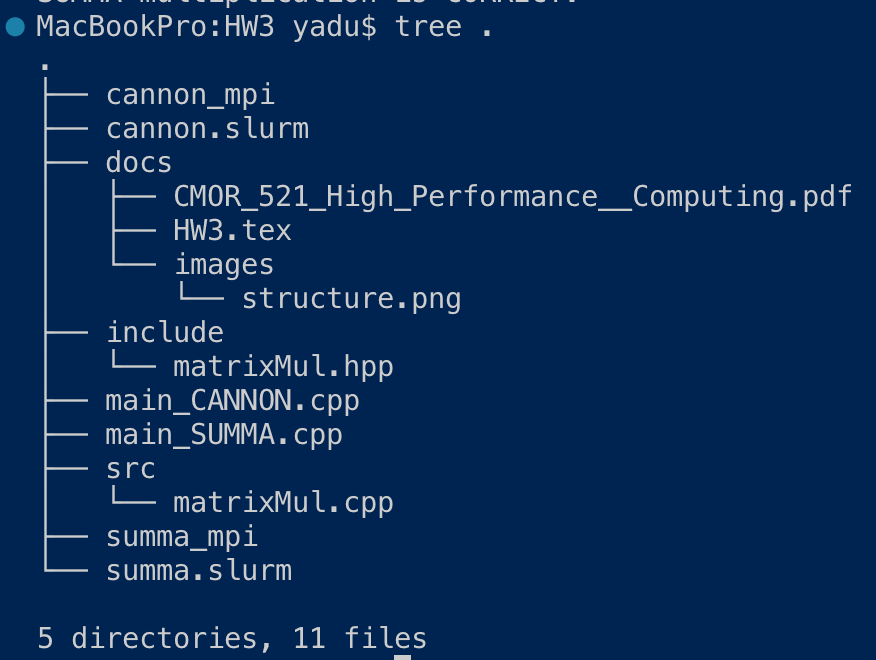
\includegraphics[width=0.3\linewidth]{Assignments/HW3/docs/images/structure.png}
    \caption{structure}
    \label{fig:structure}
\end{figure}

\begin{itemize}
    \item The \verb|include| folder and \verb|src| folder have \verb|matrixMul.hpp| and \verb|matrixMul.cpp|. In \verb|matrixMul.cpp|, there are 2 help function 
        \begin{itemize}
            \item \begin{verbatim}
                void testMul(const int N, double* serialC, double* mpiC);
            \end{verbatim}
                This function help to test that the result from both algorithms are equal to the matrix computed by serial matrix multiplication.
            \item \begin{verbatim}
                void serialMatMult(const int N, double* C, const double* A, const double* B);
            \end{verbatim}
                This function is used to compute the matrix in serial version.
        \end{itemize}
    \item The \verb|main_CANNON.cpp| and \verb|main_SUMMA.cpp| contain the Cannon's algorithm and SUMMA algorithm respectively.
    \item The \verb|cannon_mpi| and \verb|summa_mpi| are executable files. Both of them already complied by \verb|-O3| optimization flag.
    \item The \verb|cannon.slurm| and \verb|summa.slurm| are sbatch scripts.
\end{itemize}

\newpage

\section{How to Build and Run the Code (In NOTXs)}
\begin{itemize}
    \item \textbf{Build and run}
        \begin{itemize}
            \item For each algorithm you can using
            \begin{verbatim}
                sbatch summa.slurm
                sbatch cannon.slurm
            \end{verbatim}
            to run these 2 different algorithm with $2 \times 2$, $3 \times 3$, $4 \times 4$ grids with $N = 512, 768, 1024$ and $k = 64$. All these parameters can be found in \verb|*.slurm| file
        \end{itemize}
    \item \textbf{The results}
        \begin{itemize}
            \item SUMMA algorithm:
            \begin{verbatim}
        Job running on nodes: bb2u12c1,bb2u14c1
        =================================================
        === Running SUMMA on 4 procs (2×2 grid) ===
        Total error = 1.54811e-08
        SUMMA multiplication is CORRECT.
        === Running SUMMA on 9 procs (3×3 grid) ===
        Total error = 7.07518e-08
        SUMMA multiplication is CORRECT.
        === Running SUMMA on 16 procs (4×4 grid) ===
        Total error = 1.72552e-07
        SUMMA multiplication is CORRECT.
        All runs complete.
            \end{verbatim}
            \item Cannon's algorithm:
            \begin{verbatim}
        Job running on nodes: bb2u12c1,bb2u14c1
        =================================================
        === Running CANNON on 4 procs (2×2 grid) ===
        Total error = 1.1352e-08
        SUMMA multiplication is CORRECT.
        === Running CANNON on 9 procs (3×3 grid) ===
        Total error = 6.90912e-08
        SUMMA multiplication is CORRECT.
        === Running CANNON on 16 procs (4×4 grid) ===
        Total error = 1.62022e-07
        SUMMA multiplication is CORRECT.
        All runs complete.
            \end{verbatim}
        \end{itemize}
\end{itemize}
\end{document}